\chapter{Implementation}
\label{chap:impl}

\section{\Rzk{} Language Server and VS Code extesion}

In this section, we describe the implementation of the language server
and the VS Code extension for the \Rzk{} proof assistant.
The language server has direct access to the proof assistant internals,
including the typechecking algorithm and the internal abstract syntax representation,
and provides an interface conforming to the Language Server Protocol.
The VS Code extension then acts as a intermediary between the editor (VS Code)
and the language server, to bring the interactive capabilities to the user.

\subsection{Features}

% TODO: move this subsection to the requirements/design chapter?

We subject the language server to support the features specified below.

\subsubsection{Intuitive Interface and Syntax Highlighting.}

The VS Code extension introduces an intuitive interface that aligns with
the expectations of mathematicians and computer scientists.
Users benefit from clear and accessible navigation,
enabling efficient exploration of HoTT-based structures.
Furthermore, the extension provides syntax and semantic highlighting,
enhancing code readability, and facilitating error detection.

\begin{figure}
  \centering
  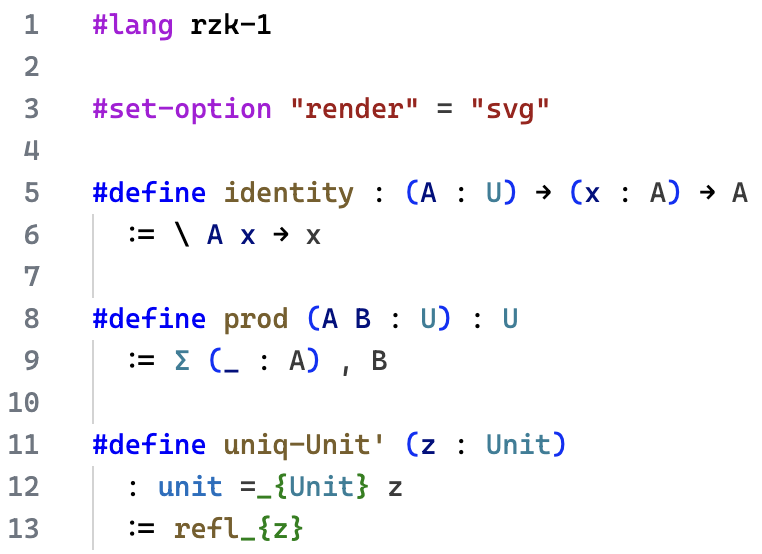
\includegraphics[width=0.7\textwidth]{figs/syntax-highlighting.png}
  \caption{Syntax/Semantic highlighting in VS Code.}
  \label{figure:syntax-highlighting}
\end{figure}

\subsubsection{Code Completion and Suggestions.}

\Rzk{}'s VS Code extension leverages the LSP to offer intelligent code completion
and context-aware suggestions. As users work with \Rzk{}, the extension assists
in writing code more efficiently by providing relevant suggestions, reducing
the likelihood of syntax errors, and accelerating the development process.

\begin{figure}
  \centering
  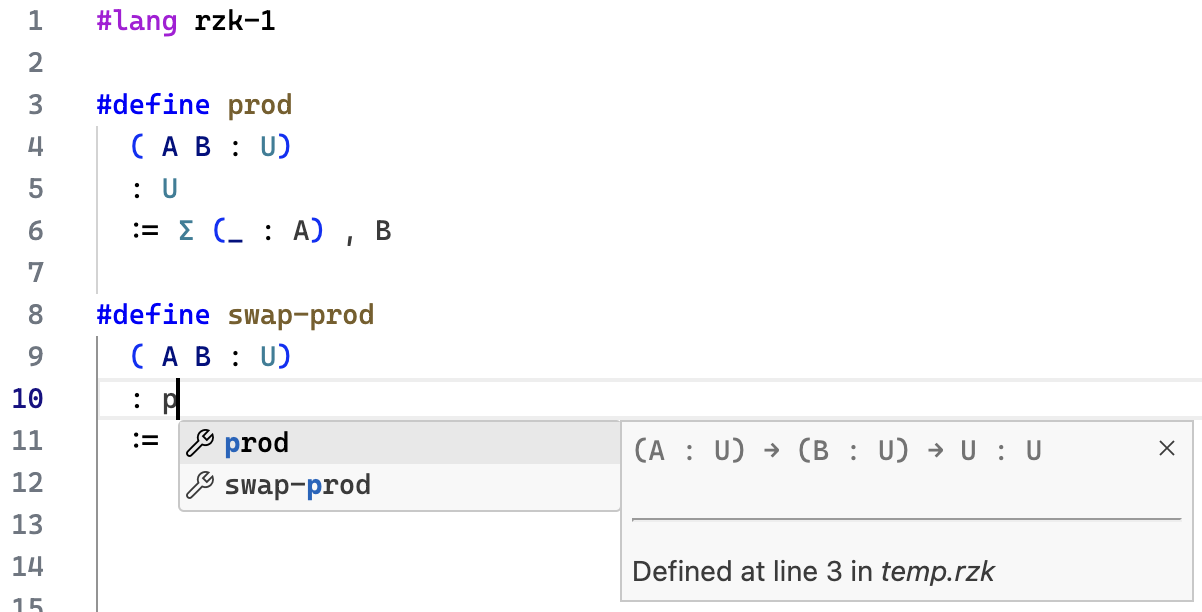
\includegraphics[width=0.7\textwidth]{figs/code-completions.png}
  \caption{Code completions in VS Code.}
  \label{figure:code-completions}
\end{figure}

\subsubsection{Real-time Error Checking.}

One of the extension's notable strengths lies in its ability to perform real-time error checking.
As users input and modify code, the language server continuously analyzes it,
reporting back any type errors or other issues with the proof.
This proactive error checking mechanism empowers users to identify and rectify issues promptly,
fostering the creation of mathematically sound programs.

\begin{figure}
  \centering
  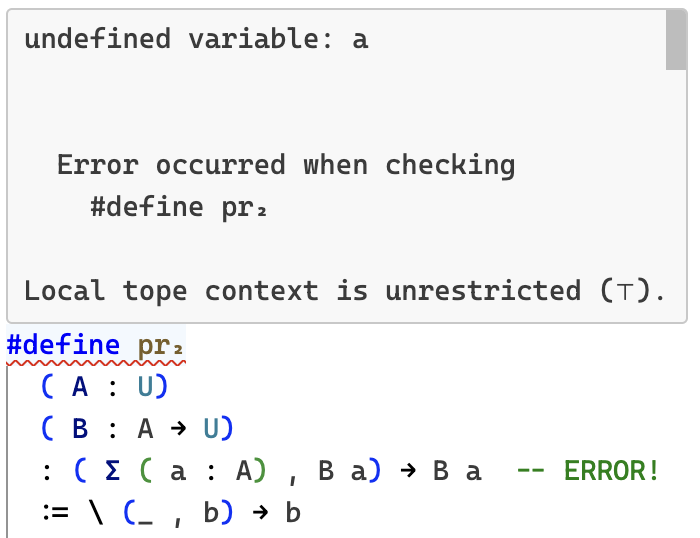
\includegraphics[width=0.7\textwidth]{figs/diagnostic-message.png}
  \caption{An error diagnostic message in VS Code.}
  \label{figure:diagnostic-message}
\end{figure}

\subsection{VS Code extension}

To bring about these features to the users, a thin wrapper around the language server in the form of a VS Code extension is necessary.
Additionally, the extension manages the installation of the language server itself on all major operating systems (Windows, macOS, and Ubuntu)
powered by pre-built binaries attached to releases on GitHub,
in addition to facilitating building the language server from source on platforms
for which pre-built binaries are not available.
The source code of the extension is available on the GitHub repository\footnote{
  \url{https://github.com/rzk-lang/vscode-rzk}},
and the extension itself is available on the Visual Studio Marketplace\footnote{
  \url{https://marketplace.visualstudio.com/items?itemName=NikolaiKudasovfizruk.rzk-1-experimental-highlighting}}.
and on the Open VSX registry\footnote{
  \url{https://open-vsx.org/extension/NikolaiKudasovfizruk/rzk-1-experimental-highlighting}},
as well as a pre-built binary on the GitHub releases page\footnote{
  \url{https://github.com/rzk-lang/vscode-rzk/releases}}.

\subsubsection{Installation and Activation}

Once the extension is activated, it checks if the \Rzk{} executable is available on the system's
\texttt{PATH} and if not, checks if it was previously downloaded to the extension's local storage directory.
If neither are available, it prompts the user to download the latest compatible binary from the GitHub
releases page and saves it in the local storage directory.
The user can override this behavior by specifying a custom path to the language server binary.

\begin{listing}
  \begin{minted}{typescript}
function locateRzk(context: vscode.ExtensionContext) {
  let path = vscode.workspace.getConfiguration().get<string>('rzk.path') ?? '';
  // Probe 1 - extension settings
  if (path) {
    const result = spawnSync(path, ['version']);
    if (result.status === 0) {
      return path;
    } else {
      output.appendLine(
        'The configured `rzk.path` option does not point to a valid rzk executable'
      );
    }
  }

  // Probe 2 - global PATH
  const binExtension = process.platform === 'win32' ? '.exe' : '';
  path = 'rzk' + binExtension;
  let result = spawnSync(path, ['version']);
  if (result.status === 0) {
    return path;
  } else {
    output.appendLine('Cannot find rzk globally');
  }

  // Probe 3 - extension storage bin folder
  path = vscode.Uri.joinPath(
    context.globalStorageUri,
    'bin',
    'rzk' + binExtension
  ).fsPath;
  result = spawnSync(path, ['version']);
  if (result.status === 0) { return path; }

  return null;
}
  \end{minted}
  \caption{The function responsible for finding where \Rzk{} is installed}
\end{listing}

To download a pre-built binary of \Rzk{}, the extension queries the available releases on the
GitHub repository and finds the latest release compatible with the installed version of the extension.
Compatibility is determined by defining a semver \cite{Preston2013semantic} range in the extension's source code,
which is then used to filter the releases and find the latest one that satisfies the range.

\begin{listing}
  \begin{minted}{typescript}
import semver from 'semver';
import type { RestEndpointMethodTypes } from '@octokit/rest';

/** In semver range format */
const supportedRzkVersions = '>=0.6.0 <1.0.0';

type GitHubRelease =
  RestEndpointMethodTypes['repos']['listReleases']['response']['data'][number];

/**
 * Checks whether the given rzk version is compatible with the extension
 * @param version A version string, e.g. "1.3.2" or "v0.4.1.1"
 */
export function isCompatibleVersion(version: string) {
  return semver.satisfies(semver.coerce(version) ?? '', supportedRzkVersions);
}
  \end{minted}
  \caption{Version compatibility check in the VS Code extension.}
  \label{code:ext-version}
\end{listing}

Then, the extension downloads the binary using Octokit SDK and extracts the tar archive to the local storage directory.

After that, the extension simply starts the language server in a separate process and establishes a connection to it,
and the rest is handled by VS Code and the language server.

\subsubsection{Configuration}

The extension provides configuration options to the user to customize the behavior of the extension.
The user can specify the path to the \Rzk{} executable, which is useful for users who have the executable installed in a non-standard location, as well as for testing purposes.
The user can also enable or disable the formatting feature and choose whether to receive pre-release versions of \Rzk{}.

\begin{figure}
  \centering
  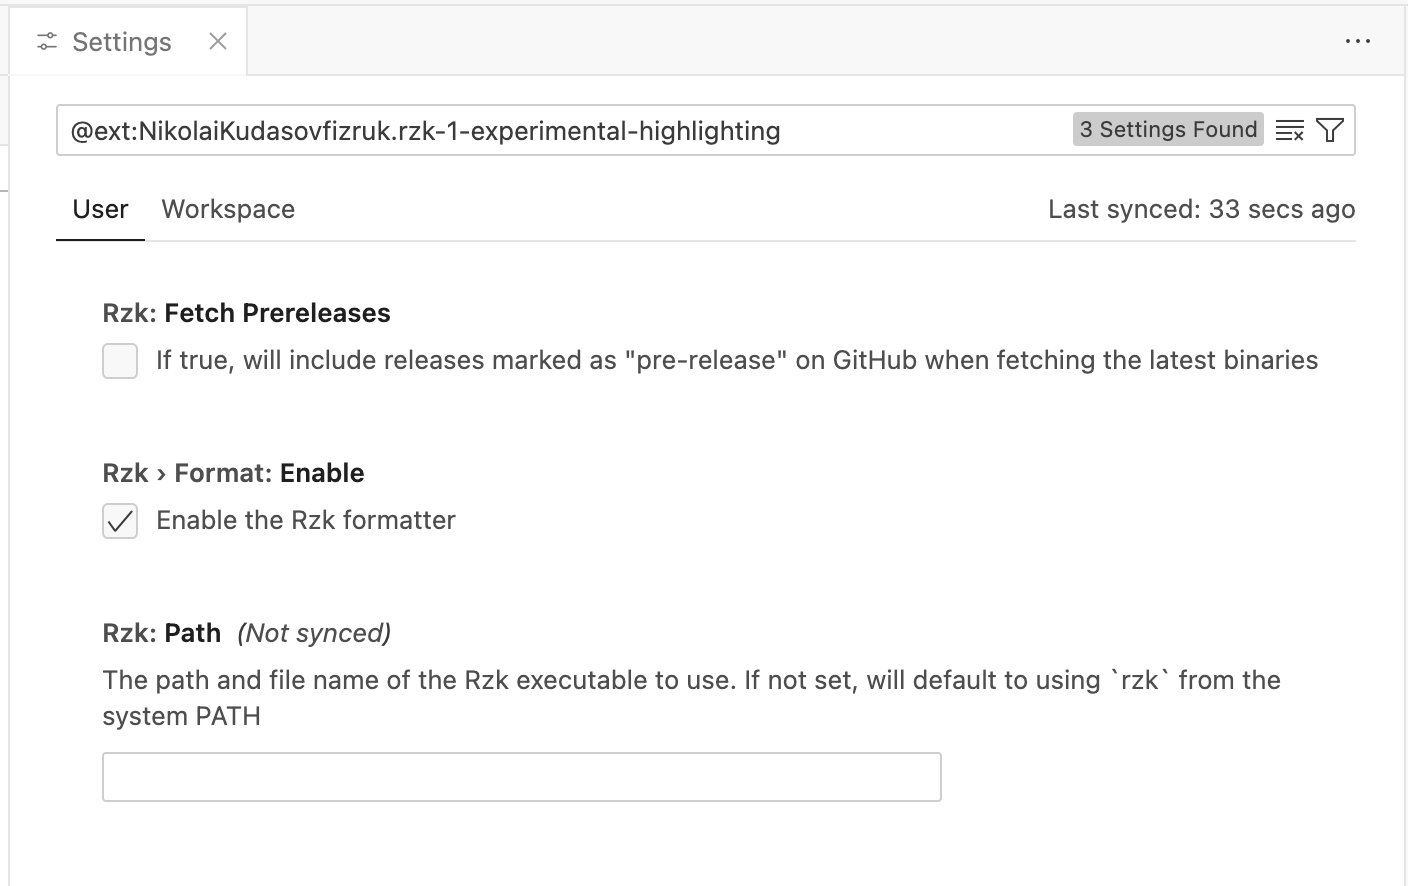
\includegraphics[width=0.8\textwidth]{figs/rzk-vscode-settings.png}
  \caption{The extension configuration section in VS Code.}
  \label{figure:vscode-settings}
\end{figure}

This is achieved using the configuration\footnote{
  \url{https://code.visualstudio.com/api/references/contribution-points\#contributes.configuration}}
field in \texttt{package.json}

\subsection{\Rzk{} Language Server}

At the core of the \Rzk{} tool suite is the language server that powers all the editor features that make it pleasant to develop proofs in \Rzk{}. In particular, it currently supports semantic highlighting, diagnostic messages, and text completion. Additionally, progress reporting for long-running processes (such as type-checking for large projects) is currently under work.

For the first versions of the language server, it is shipped as part of the \Rzk{} proof assistant itself under a different subcommand, but it is planned to decouple both components and have the language server depend on the core library. They are implemented in the Haskell programming language using the \texttt{lsp}\footnote{\url{https://hackage.haskell.org/package/lsp}} package.

It is also worth mentioning that the language server is designed to be compatible
with any other editor that supports LSP, not just VS Code.
In particular, users have reported success in integrating it with the NeoVim editor,
and it is planned to be tested with other editors as well.

The language server currently supports the features outlined in the following sections, with more features planned for the future.

\subsubsection{Diagnostics Reporting}

Every time the user saves a file that is part of a formalization project, the language server runs the typechecker
on the project and reports any errors or warnings that it finds, caching the results to speed up future typechecks.
The errors and warnings are sent as diagnostic messages via the LSP protocol to the editor,
which then displays them in the editor's interface.
This feature is crucial for the users to be able to quickly identify and fix any errors in their proofs.
These messages are displayed on the location in the file where the error occurred,
and contain a useful message that explains what went wrong with all the necessary context.

\subsubsection{Text Completion}

The language server also provides text completion suggestions to the user as they type.
These suggestions are context-aware and are based on the current cursor position in the file.
They include previously defined proof identifiers, their types, and their definition locations.

\subsubsection{Semantic Highlighting}

Another feature that the language server provides is semantic highlighting, which colors different parts of the code
based on their meaning.
This differs from syntax highlighting in that it is smarter and can use more information in determining a token's type (and hence color),
This is because it uses information from the parser, and not just from the lexer.
It can also use additional information from the typechecker to determine the type of a token,
but this is currently not implemented since it was not deemed necessary.

\subsubsection{Formatting}

The language server also provides a formatting feature that allows the user to format their code according to a predefined style.
This is useful for keeping the codebase consistent and readable, and is especially useful when working in a team.
The formatter catches common style issues such as indentation, spacing, and line breaks,
and automatically fixes them according to the predefined style.

A separate CLI subcommand is available to expose this feature outside of the language server as well.

\section{Satellite Tools}

% TODO

\subsection{MkDocs Plugin}

The \texttt{rzk-mkdocs-plugin} is a Python package that provides a plugin for the MkDocs static site generator.

\subsection{GitHub Action}

The \texttt{rzk-github-action} is a GitHub Action that can be used to run the \Rzk{} proof assistant on a GitHub repository.
